\section{Evolutionärer Algorithmus}\label{sec:evol-alg}
Für den Algorithmus wird angenommen,
dass die eine Liste der möglichen Spendetermine wie folgt eingegeben wird:
\begin{table}[ht]
    \begin{center}
        \begin{tabular}{l|c|c|c|c}
            PLZ     & Ort               &  Straße               & Datum     & Distanz   \\
            \hline
            12345   & Musterstadt       & Hauptstraße 42        & 5.3.2019  & 6.31      \\
            04711   & Beispieldorf      & Spenderstraße. 13     & 894.2019  & 20.42     \\
        \end{tabular}
    \end{center}
    \caption{Beispieldaten}
\end{table}


Für den Algorithmus selbst sind hierbei lediglich die letzen beiden Merkmale notwendig.
Die anderen Merkmale dienen der finalen Darstellung für den Anwender.

Das Problem ähnelt stark dem bekannten \emph{Knappsackproblem}.
Dort wird versucht den Gesamtwert der mitgenommenen Gegenstände zu maximieren
und dabei die vorgegebenen Gewichtsgrenzen einzuhalten.

Entsprechend soll in dem hier beschriebenen Fall die Anzahl der besuchten Spendetermine unter
Einhaltung bestimmter Regeln maximiert werden.
Ergänzt wird diesen Problem durch die Minimierung der zurückgelegten Strecke.

\subsection{Genstring}
Wie auch bei einem Knappsackproblem üblich wird der Genstring wird als Bitstring modelliert.
Somit gilt:

\begin{equation}
    \label{eqn:genstring}
    \begin{split}
        x_i &\in \{ 0,1 \} \\
        x_i &= 1 \Rightarrow \text{Termin $i$ wird wahrgenommen} \\
        x   &= b_1b_2...b_n \in \{0,1\}^n\text{ mit $n = $ Anzahl der eingegebenen Termine}
    \end{split}
\end{equation}

\subsection{Bewertungsfunktion}
Die Bewertungsfunktion hat das Ziel die Anzahl der besuchten Termine zu maximieren und die Gesamtstrecke zu minimieren.
Dies soll unter Beachtung der bereits vorgestellten Bedingungen geschehen.

Im Vergleich zu beispielsweiße einer Produktionsplanung gibt es bei den Bedingungen keinen Spielraum.
In einer Produktionsplanung ist es möglicherweiße gestattet die maximale Anzahl der verplanten Stunden zu überschreiten.
Dies wird in der Fitness entsprechend bestraft. Aber sollte das beste Ergebnis Überstunden enthalten ist es dennoch ein gültiges Ergebnis.

Die Bedingungen für das Blutspenden sind jedoch \enquote{harte} Bedingungen.
Das heißt, dass beispielsweiße keine Spende möglich ist, wenn die letze Spende erst 55 Tage her ist und nicht die geforderten 56.
Um solche Ergebnisse zu verhindern ist de Fitness für diese Gene $0$.
Da die Anzahl der Spenden innerhalb von 12 Monateg geschlechterspezifisch ist,
fließt diese Zahl durch die Konstante $c$ in die Berechnung mit ein.

Anzahl der besuchten Termine und eine minimale Strecke sind zwei sich entgegenstehende Ziele.
Würde mann keinen der Termine wahrnehmen, so wäre die Gesamtstrecke gleich $0$ und damit optimal.

Daher wird eine Gewichtung der beiden Merkmale durchgeführt.
$w \in [0,1]$ steht hierbei für die Gewichtung der Anzahl.
Entsprechend ist $(1-w)$ die Gewichtung für die Strecke.
Um sicherzustellen dass das Gewicht für beide Merkmale den gleichen Einfluss besitzt,
werden die jeweiligen Bewertungen auf den Bereich $[0,1]$ normiert.
Für die Anzahl geschieht dies durch eine Division mit $c$.

Das Normieren der Strecke ist hierbei komplexer.
Deren Bewertung wird mit $(1 - \frac{\sum x_i * d_i}{max(d)t* \sum x_i})$ berechnet.
Durch den Bruch wird der durchschnittliche Abstand zu maximal möglichen Strecke ($max(d)$) berechnet.
Am anschaulichsten erklärt sich diese Formel durch Betrachtung der Grenzfälle:
\begin{table}[ht]% Try here, and then top
    \begin{center}
        \begin{tabular}{l|c|c}
            Fall                            & $\cfrac{\sum x_i * d_i}{max(d) * \sum x_i}$  &  Bewertung \\
            \hline
            $\forall x_i = 1: d_i = max(d)$ & $1$                                           & $0$       \\
            $\forall x_i = 1: d_i = 0$      & $0$                                           & $1$       \\
        \end{tabular}
    \end{center}
    \caption{Grenzfälle Bewertung der Strecke}
  \end{table}

Insgesamt lässt sich die Fitness eines Gens nach Formel \ref{eqn:fitness} berechnen.
Die Funktion $B(x)$ bestimmt hierbei, ob die Nebenbedingungen erfüllt sind.

\begin{equation}
    \label{eqn:fitness}
    f(x)=
    \begin{cases}
        0,              & \text{wenn } B(x) = 0 \\
        w * \cfrac{\sum x_i}{c} + (1 - w) * \left(1 - \cfrac{\sum x_i * d_i}{max(d) * \sum x_i}\right) & \text{sonst}
    \end{cases}
\end{equation}

In Formel \ref{eqn:bedingung} ist die Formel für die Bedingungen dargestellt.
$t_i$ steht hierbei für das Datum eines Spendetermins.
Ist das Ergebnis $1$ so gelten die Bedingungen als erfüllt.



\begin{multline}
    \label{eqn:bedingung}
    B(x)=
    \begin{cases}
        0, & \text{wenn } \exists x_i \in x : x_i = 1  \wedge \\
           & \hspace{10ex} \lvert \{ x_j\in x \mid x_j = 1 \wedge i < j \wedge t_j - t_i <= 1y  \} \rvert > c   \\
        0, & \text{wenn } \exists x_i, x_j \in x : \left( (x_i = x_j = 1) \wedge (i < j) \wedge (t_j - t_i < 56d) \right)    \\
        1  & \text{sonst}
    \end{cases}
\end{multline}

Durch die verhältnismäßig strengen Bedingungen ist mit einer hohen Anazhl an \emph{Totgeburten} zu rechnen.
Kompensiert wird dies durch eine große Population um ausreichend \enquote{gesunde} Gene zur späteren Rekombination zu erhalten.




\subsection{Kombination}\label{sec:evol-alg-kombi}
Zwei Gene werden durch einen sogenannten \emph{1-Point Crossover} \cite{AJ2015}.
Hierzu werden die Bitstrings der Eltern an einer zufälligen Stelle getrennt und die Teilstrings untereinander getauscht.
Folgende Tabelle zeigt beispielhaft den Crossover an Position 4 von zwei Bitstirngs der Länge 9:

\begin{table}[ht]
    \begin{center}
        \begin{tabular}{l c}
            Elternteil 1 & \colorbox{lime!30}{$1010$~}$\mid$\colorbox{lime!30}{ $10010$} \\
            Elternteil 2 & \colorbox{cyan!30}{$1011$~}$\mid$\colorbox{cyan!30}{ $10110$} \\
            \hline
            Kind 1       & \colorbox{lime!30}{$1010$~}$\mid$\colorbox{cyan!30}{ $10110$} \\
            Kind 2       & \colorbox{cyan!30}{$1011$~}$\mid$\colorbox{lime!30}{ $10010$} \\
        \end{tabular}
    \end{center}
    \caption{1-Point Crossover (nach \cite{AJ2015})}
\end{table}

Die Auswahl der zu kombinierenden Eltern geschieht durch eine \emph{Tournament Selection} mit vier Teilnehmern.
Wie in \autoref{fig:tournament} dargestellt werden erst jeweils zwei der vier Teilnehmer miteinander verglichen.
Jeweils die besten beiden werden dann nochmals miteinander Verglichen um den Sieger zu ermittelt.

\begin{figure}[h]
    \centering
    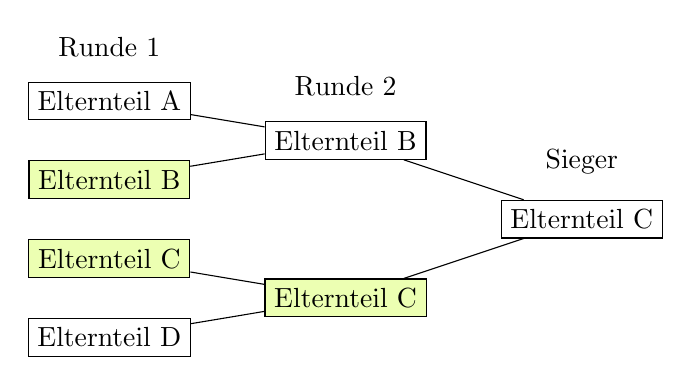
\begin{tikzpicture}
        [
           every node/.style={rectangle,draw},
           level distance=3cm
        ]
        \tikzstyle{level 1}=[sibling distance=20mm]
        \tikzstyle{level 2}=[sibling distance=10mm]
        \node[label={[label distance=0.2cm]90:Sieger}] {Elternteil C} [grow'=left]
        child {node[fill=lime!30]{Elternteil C}
            child {node{Elternteil D}}
            child {node[fill=lime!30]{Elternteil C}}
        }
        child {node[label={[label distance=0.2cm]90:Runde 2}]{Elternteil B}
            child {node[fill=lime!30]{Elternteil B}}
            child {node[label={[label distance=0.2cm]90:Runde 1}]{Elternteil A}}
        };
    \end{tikzpicture}
    \caption{Beispiel eines Tournaments}
    \label{fig:tournament}
\end{figure}

\subsection{Mutationen}
In einem Knappsackproblem ist eine Bitinversion eine übliche Mutation.
Für das Blutspende-Problem bringt eine zufällige Bitinversion mit sehr hoher Wahrscheinlichkeit
eine Reduktion der Fitness mit sich.

Wird ein aktives Bit deaktiviert, so sinkt damit logischerweiße die Anzahl der wahrgenommenen Termine und damit die Fitness.
Wird ein inaktives Bit aktiviert, so ist die Wahrscheinlichkeit hoch, dass eine der Bedingungen verletzt wird.

Daher wird zur Mutation kein Bit invertiert sondern zufällig in seiner unmittelbaren Nachbarschaft verschoben.
Die Weite und Richtung der Verschiebung wird zufäiig ermittelt. Als maximal mögliche Verschiebung wird die Schrittweite angenommen.
Dise wird inital gesetzt und dann mittels der $\frac{1}{5}$-Regel iterativ angepasst.

Die Regel beasgt, dass die Schrittweite erhöht wird, falls mehr als $\frac{1}{5}$ der Mutationen besser sind als ihre Ursprungsgene
und verringert wird, falls weniger als $\frac{1}{5}$ erfolgreich sind.

Da positive Bits nur Verschoben und keine negativen Bits aktiviert werden,
erhöht sich die Anazhl der besuchten Termine nicht durch die Mutation.
Dies geschieht jedoch mit der vorherigen Rekombination zweier Gene.

\subsection{Initiale Population}
Initial wird die Population erzeugt,
indem für jedes Gen drei zufällige Bits gesetzt werden.
Um die Wahrscheinlichkeit zu reduzieren, dass diese Bits zu Nah zueinander sind,
wird jedes der Bits auf ein Drittel des Genstrings beschränkt.

Zum Vergleich wurden 100 mal jeweils Populationen von 1000 Genen mit beiden Verfahren erzeugt.
Der Versuch zeigt, dass mit ohne diese Beschränkung lediglich etwa 35\% der Gene die Bedingungen erfüllen.
Die Beschränkung hebt den Anteil der gültigen Gene auf etwa 80\%.

Durch eine hohe Zahl an Totgeburten hat dies den Nachteil,
dass anfangs nur wenige \enquote{nützliche} Gene zur Verfügung stehen.
Dies wird durch eine hohe Populationszahl kompensiert.
Ein prototypisches Programm, welches in \autoref{sec:prototyp} vorgestellt wird,
zeigt, dass eine Population von 1000 hierfür ausreicht.

 \subsection{Population}
Die Evolution geschieht nach folgenden Regeln.
Die entsprechenden Parameter können im Programm variiert werden.
\begin{itemize}
    \item Eine \emph{Elite} der fittesten Gene \enquote{überlebt} eine Generation
    \item Die restlichen Gene der nächsten Generation werden durch Kombination erzeugt.
    \begin{itemize}
        \item Hierfür kommen nach dem in \autoref{sec:evol-alg-kombi} vorgestellten Verfahren alle Gene der aktuellen Generation in Frage.
        \item Zusätzlich wird ein neu erzeugtes Gen mit einer gewissen Wahrscheinlichkeit mutiert.
    \end{itemize}
    \item Nach Kombination und Mutation werden alle Gene, welche nicht die Bedingungen erfüllen aus der Population entfernt.
    \item Der gesamte Algorithmus endet, wenn die durchschnittliche und die beste Fitness mit gegebener Präzision identisch sind oder spätestens nach einer maximalen Anzahl von Durchläufen
\end{itemize}